\section{Динамика материальной точки}
%Сив73
\AddProb В лифте установлены пружинные весы, на которых подвешено тело массы 1 кг. Что будут показывать весы, если лифт: 1) движется вверх с ускорением 5 м/с\textsuperscript{2}, направленным вниз; 2) движется вниз с ускорением 5 м/с\textsuperscript{2}, направленным вверх?

%Сив76
\begin{wrapfigure}[10]{r}{4cm}
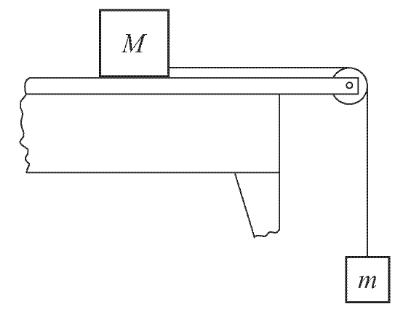
\includegraphics[width=0.3\textwidth]{block2Bodies.png}
\caption{}
\label{block2Bodies}
\end{wrapfigure}
\AddProb На гладкой горизонтальной плоскости находится тело массы $М$ (рис. \ref{block2Bodies}). Другое тело массы $m$ подвешено на нити, перекинутой через блок и привязанной к телу массы $М$. Найти ускорения тел и натяжение нити. Трением тела массы $М$ о плоскость и трением в блоке, а также массами блока и нити пренебречь.
%Сив79
\AddProb По наклонной плоскости с углом наклона $\alpha$ скользит тело. Сила трения между телом и плоскостью пропорциональна силе нормального давления тела на плоскость и не зависит от скорости тела. Коэффициент трения между трущимися поверхностями тела и плоскости равен $\mu$. Найти ускорение $a$, с которым скользит тело.

\begin{figure}[h]
\centering
\begin{subfigure}{.43\textwidth}
  \centering
  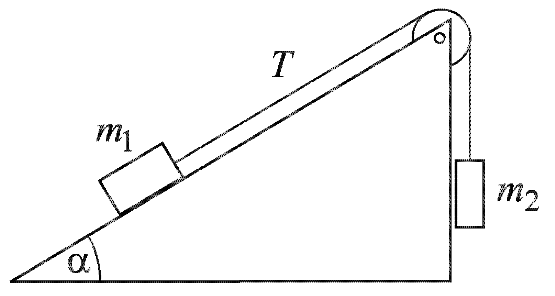
\includegraphics[width=1.0\linewidth]{inclinedPlane.png}
  \caption{}
  \label{inclinedPlane}
\end{subfigure}%
\begin{subfigure}{.57\textwidth}
  \centering
  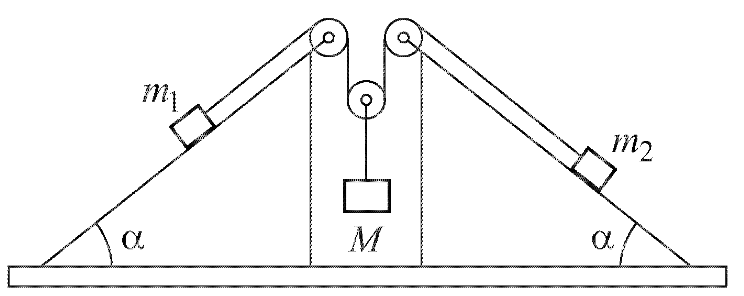
\includegraphics[width=1.0\linewidth]{2InclinedPlanes.png}
  \caption{}
  \label{2InclinedPlanes}
\end{subfigure}
\caption{}
\end{figure}

%Сив96
\AddProb На верхнем краю идеально гладкой наклонной плоскости укреплен блок, через который перекинута нить (рис. \ref{inclinedPlane}). На одном ее конце привязан груз с массой $m_1$, лежащий на наклонной плоскости. На другом конце висит груз с массой $m_2$. С каким ускорением $a$ движутся грузы и каково натяжение $Т$ нити? Наклонная плоскость образует с горизонтом угол $\alpha$.
%Сив97
\AddProb Определить ускорение массы $М$ в системе, изображенной на рис. \ref{2InclinedPlanes}. Массой блоков и силами трения можно пренебречь. Клинья считать закрепленными жестко.

%Сив78
\begin{wrapfigure}[13]{r}{6cm}
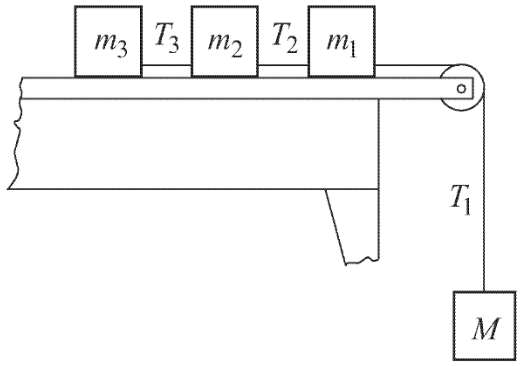
\includegraphics[width=0.5\textwidth]{4Bodies.png}
\caption{}
\label{4Bodies}
\end{wrapfigure}
\AddProb На гладкую горизонтальную плоскость помещены три массы $m_1$, $m_2$, $m_3$ связанные нитями между собой и с массой $M$, привязанной к нити, перекинутой через блок (рис. \ref{4Bodies}). 1) Найти ускорение $a$ системы; 2) найти натяжение всех нитей. Трением тел о плоскость и трением в блоке, а также массами блока и нити пренебречь.
%Сив80
\AddProb Два одинаковых тела связаны нитью и лежат на идеально гладком горизонтальном столе, так что нить представляет собой прямую линию. Нить может выдерживать натяжение с силой не	более 100 Н. Какую горизонтальную силу $F$ следует приложить к одному из тел, чтобы нить оборвалась?
%Сив85-86
\AddProb Лошадь равномерно тянет сани. Рассмотреть взаимодействие трех тел: лошади, саней и поверхности земли. Начертить векторы сил, действующих на каждое из этих тел в отдельности. Найти величину всех сил, если лошадь и сани движутся с ускорением $a = 20$ см/с\textsuperscript{2}. Масса саней с грузом $M = 0,5$ т, масса лошади $m = 0,35$ т и коэффициент трения саней о снег $\mu = 0,2$.
%Сив90
\AddProb Воздушный шар массы $M$ опускается с постоянной скоростью. Какое количество балласта $m$ надо выбросить, чтобы шар начал подниматься с той же скоростью? Подъемную силу $Р$ шара считать постоянной.

\begin{figure}[h]
\centering
\begin{subfigure}{.3\textwidth}
  \centering
  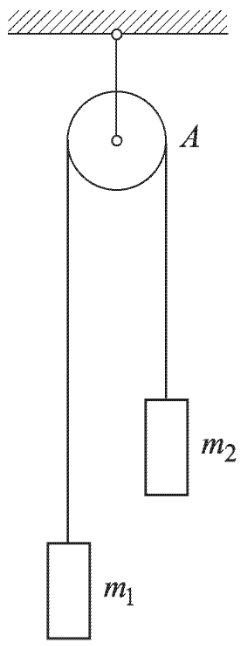
\includegraphics[width=0.7\linewidth]{Atwood.png}
  \caption{}
  \label{Atwood}
\end{subfigure}%
\begin{subfigure}{.3\textwidth}
  \centering
  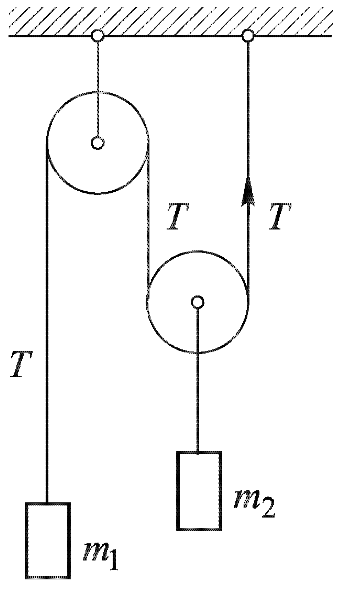
\includegraphics[width=1.0\linewidth]{Atwood2.png}
  \caption{}
  \label{Atwood2}
\end{subfigure}
\begin{subfigure}{.3\textwidth}
  \centering
  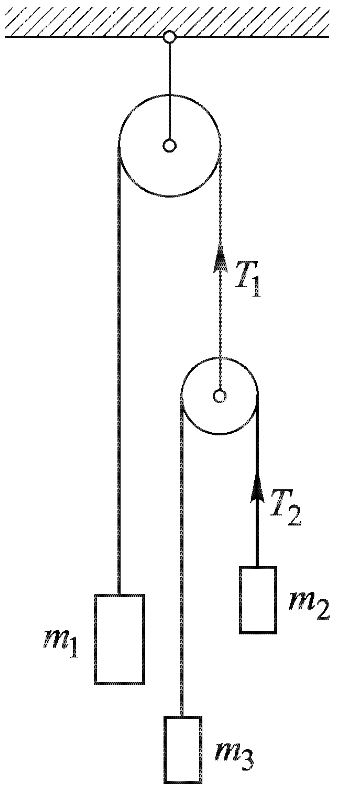
\includegraphics[width=1.0\linewidth]{Atwood3.png}
  \caption{}
  \label{Atwood3}
\end{subfigure}
\caption{}
\end{figure}
%Сив95
\AddProb Простейшую машину Атвуда, служащую для проверки законов равноускоренного движения, можно схематически представить так: на нити, перекинутой через блок $A$, подвешены две неравные массы, $m_1$
и $m_2$ (рис. \ref{Atwood}). Найти ускорение масс, натяжение нити $T$ и силу $F$, действующую на ось блока этой машины. Блок и нить считать невесомыми, трения в оси блока не учитывать.
%Сив103
\AddProb Найти ускорения $a_1$ и $a_2$ масс $m_1$ и $m_2$ и натяжение нити $Т$ в системе, изображенной на рис. \ref{Atwood2}. Массой блоков и нитей пренебречь.
%Сив104
\AddProb Найти ускорение массы $m_1$ и натяжения нитей $T_1$ и $T_2$ в системе, изображенной на рис. \ref{Atwood3}. Массой блоков и нитей пренебречь, сил трения не учитывать.
%Иродов1.65
\AddProb Небольшое тело пустили вверх по наклонной плоскости, составляющей угол $\alpha  = 15^{\circ}$ с горизонтом. Найти коэффициент трения, если время подъема тела оказалось в $k = 2,0$ раза меньше времени спуска.
%Сив112
\AddProb Как будет изменяться скорость тела массы $m$, движущегося вертикально вверх с начальной скоростью $v_0$, если можно считать, что сила сопротивления воздуха пропорциональна скорости тела $F = -rv$, где $r$ -- постоянный коэффициент сопротивления?

\clearpage